\chapter{Anleitung für Studierende}
\label{sec:chap3}

\section{Kursübersicht}

Meldet sich ein Student an, wird er nach dem Login auf die Kursübersicht weitergeleitet (beispielhaft in Abbildung \ref{fib:kursübersicht_student}). Hier werden alle Kurse angezeigt, in denen der Nutzer Mitglied ist.
Auf diese Ansicht kann der Nutzer zu jeder Zeit über die Schaltfläche \glqq Kursübersicht\grqq zu dieser Ansicht zurückkommen. 

\begin{figure}[h]
\centering
\includegraphics[height=.5\textwidth]{kursübersicht_dozent.png}
\caption{Kursübersicht eines Dozenten in der Anwendung eCourse}
\label{fib:kursübersicht_student}
\end{figure}

In der ausklappten Kursansicht (siehe beispielhaft Abbildung \ref{fib:kursübersicht_student_aus} )sieht der Nutzer den Dozenten des Kurses sowie alle Aufgaben zum Kurs. Möchte der Nutzer genauere Informationen zu einer bestimmten Aufgabe erhalten, erhält er diese durch betätigen der Schaltfläche \glqq Anzeigen\grqq. Auf der dann angezeigten Seite kann die Aufgabenstellung heruntergeladen werden und Lösungen hochgeladen werden. Mehr dazu in Kapitel \ref{sec:aufg}.

\begin{figure}[h]
\centering
\includegraphics[height=.5\textwidth]{kursübersicht_student_ausgeklappt.png}
\caption{Ausgeklappte Kursübersicht eines Studenten in der Anwendung eCourse}
\label{fib:kursübersicht_student_aus}
\end{figure}

\section{Aufgaben}
\label{sec:aufg}
Um die Lösung für eine Aufgabe abzugeben muss der Nutzer über die ausgeklappte Kursübersicht auf die Aufgabe anzeigen. Dadurch öffnet sich eine neue Seite, wie in Abbildung \ref{fib:hochladen} gezeigt. Hier kann dann durch betätigen der Schaltfläche \glqq Durchsuchen\grqq eine .pdf-Datei ausgewählt werden. Diese muss vor der Abgabe noch mit einem Namen versehen werden. Die Abgabe wird abgeschlossen durch betätigen der Schaltfläche \glqq Hochladen\grqq.
\begin{figure}[h]
\centering
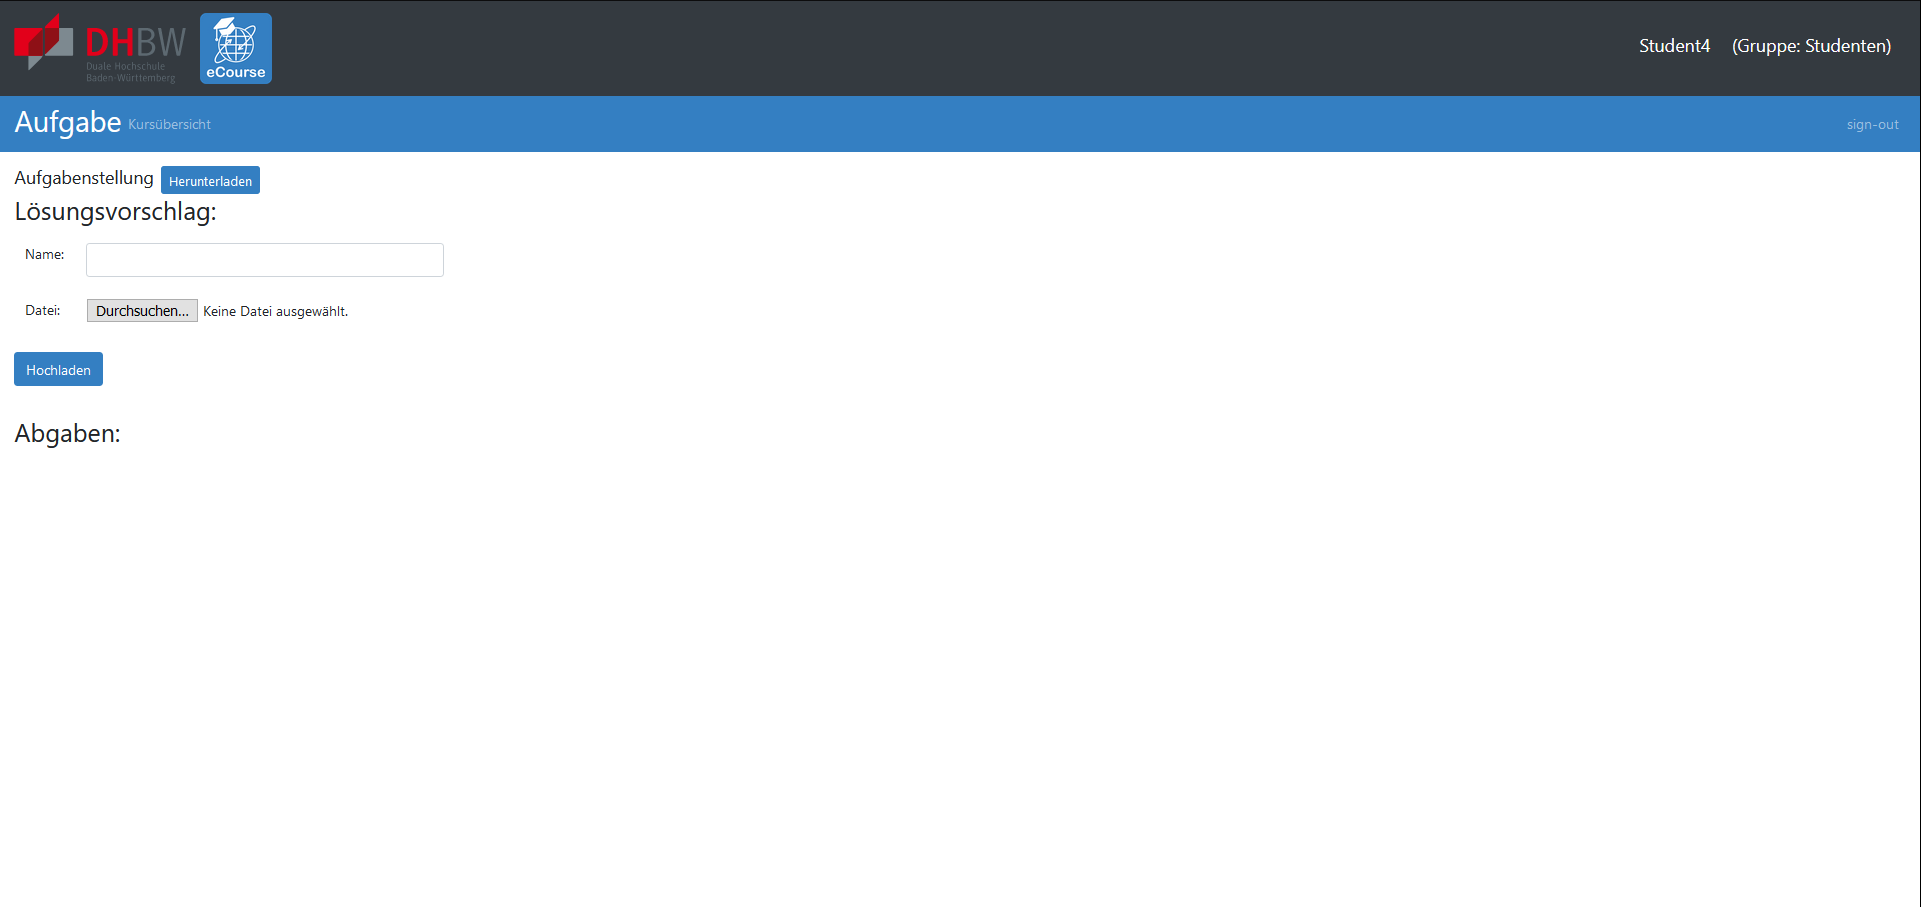
\includegraphics[height=.5\textwidth]{aufgabe_student.png}
\caption{Lösungsvorschlag hochladen durch einen Studenten in der Anwendung eCourse}
\label{fib:hochladen}
\end{figure}
